\documentclass[11pt]{article}
\usepackage[a4paper,margin=22mm]{geometry}
\usepackage{amsmath,amssymb,booktabs,longtable,array,graphicx,float,hyperref,siunitx,xcolor,microtype}
\hypersetup{colorlinks=true,linkcolor=blue!60!black,citecolor=blue!60!black,urlcolor=blue!60!black}
\sisetup{detect-all=true,per-mode=symbol}
\setlength{\parskip}{0.55em}
\setlength{\parindent}{0pt}
\title{Updated-Coil Dynamic Simulation of the Orthogonal Metglas AMCC-1000 Walter Russell Optical Dynamo Generator}
\author{Generated from \texttt{dynamic\_power\_simulator\_updated\_coils\_20260531.py}}
\date{31 May 2026}

\begin{document}
\maketitle

\begin{abstract}
This article reports a new dynamic simulation version for the updated eight-coil
and eight-cable Walter Russell Optical Dynamo Generator interpretation.  The
coil data are not the earlier placeholder lengths: the windings now use the
Grover-solved conductor lengths and turns.  Every C1--C8 conductor has the same
end-to-end active length, \SI{445.293167}{m}, while the wound portion on
each bobbin is the exact length required to produce the target branch
inductance.  The A/B ladder remains a constant-\SI{50}{\ohm} stage system
at octave frequencies \SI{16}, \SI{32}, \SI{64}, and \SI{128}{kHz}.
The orthogonal AMCC-1000 paraformer center is simulated as a separately matched
resonant magnetic subsystem.  The new simulator exports the Metglas currents,
voltages, input/output monitor signals, instantaneous power transfer, and
matched Thevenin transfer limits.
\end{abstract}

\section{Updated Coil Data Used by the Simulator}
The current simulator reads the canonical coil design CSV files from
\texttt{walter\_russell\_optical\_dynamo\_generator/outputs}.  The equal
cable-length rule is enforced by non-inductive equalizer lengths outside the
bobbin windows.

\resizebox{\textwidth}{!}{%
\begin{tabular}{lrrrrl}
\toprule
Cable & End-to-end active (m) & Wound total (m) & Equalizer (m) & Cut +3\% (m) & Wire \\
\midrule
C1 & 445.293167 & 445.293167 & 0.000000 & 459.681962 & AWG10-equivalent RF Litz, 416 x AWG36 \\
C2 & 445.293167 & 445.293167 & 0.000000 & 459.681962 & AWG10-equivalent RF Litz, 416 x AWG36 \\
C3 & 445.293167 & 185.480193 & 259.812975 & 459.681962 & AWG12-equivalent RF Litz, 262 x AWG36 \\
C4 & 445.293167 & 185.480193 & 259.812975 & 459.681962 & AWG12-equivalent RF Litz, 262 x AWG36 \\
C5 & 445.293167 & 92.147202 & 353.145966 & 459.681962 & AWG18-equivalent RF Litz, 65 x AWG36 \\
C6 & 445.293167 & 92.147202 & 353.145966 & 459.681962 & AWG18-equivalent RF Litz, 65 x AWG36 \\
C7 & 445.293167 & 92.147202 & 353.145966 & 459.681962 & AWG18-equivalent RF Litz, 65 x AWG36 \\
C8 & 445.293167 & 92.147202 & 353.145966 & 459.681962 & AWG18-equivalent RF Litz, 65 x AWG36 \\
\bottomrule
\end{tabular}
}

\resizebox{\textwidth}{!}{%
\begin{tabular}{lrllll}
\toprule
Stage & f (kHz) & Active cables & Lengths in bobbin (m) & Turns by cable & Physical L match (\%) \\
\midrule
A1 & 16.000 & C1 C2 & C1:75.937339 C2:75.937339 & C1:128.599732 C2:128.599732 & 99.999999999 \\
A2 & 32.000 & C1 C2 & C1:53.769615 C2:53.769615 & C1:91.058737 C2:91.058737 & 100.000000002 \\
A3 & 64.000 & C1 C2 C3 C4 & C1:46.469815 C2:46.469815 C3:46.370048 C4:46.370048 & C1:100.405929 C2:100.405929 C3:100.190366 C4:100.190366 & 100.000000000 \\
A4 & 128.000 & C1 C2 C3 C4 C5 C6 C7 C8 & C1:46.469815 C2:46.469815 C3:46.370048 C4:46.370048 C5:46.073601 C6:46.073601 C7:46.073601 C8:46.073601 & C1:100.405929 C2:100.405929 C3:100.190366 C4:100.190366 C5:99.549841 C6:99.549841 C7:99.549841 C8:99.549841 & 100.000000001 \\
B4 & 128.000 & C1 C2 C3 C4 C5 C6 C7 C8 & C1:46.469815 C2:46.469815 C3:46.370048 C4:46.370048 C5:46.073601 C6:46.073601 C7:46.073601 C8:46.073601 & C1:100.405929 C2:100.405929 C3:100.190366 C4:100.190366 C5:99.549841 C6:99.549841 C7:99.549841 C8:99.549841 & 100.000000001 \\
B3 & 64.000 & C1 C2 C3 C4 & C1:46.469815 C2:46.469815 C3:46.370048 C4:46.370048 & C1:100.405929 C2:100.405929 C3:100.190366 C4:100.190366 & 100.000000000 \\
B2 & 32.000 & C1 C2 & C1:53.769615 C2:53.769615 & C1:91.058737 C2:91.058737 & 100.000000002 \\
B1 & 16.000 & C1 C2 & C1:75.937339 C2:75.937339 & C1:128.599732 C2:128.599732 & 99.999999999 \\
\bottomrule
\end{tabular}
}

\resizebox{\textwidth}{!}{%
\begin{tabular}{llrrr}
\toprule
Stage & Cable & Length (m) & Turns & Grover L (uH) \\
\midrule
A1 & C1 & 75.937339 & 128.599732 & 994.718394 \\
A2 & C1 & 53.769615 & 91.058737 & 497.359197 \\
A3 & C1 & 46.469815 & 100.405929 & 497.359197 \\
A4 & C1 & 46.469815 & 100.405929 & 497.359197 \\
B4 & C1 & 46.469815 & 100.405929 & 497.359197 \\
B3 & C1 & 46.469815 & 100.405929 & 497.359197 \\
B2 & C1 & 53.769615 & 91.058737 & 497.359197 \\
B1 & C1 & 75.937339 & 128.599732 & 994.718394 \\
A1 & C2 & 75.937339 & 128.599732 & 994.718394 \\
A2 & C2 & 53.769615 & 91.058737 & 497.359197 \\
A3 & C2 & 46.469815 & 100.405929 & 497.359197 \\
A4 & C2 & 46.469815 & 100.405929 & 497.359197 \\
B4 & C2 & 46.469815 & 100.405929 & 497.359197 \\
B3 & C2 & 46.469815 & 100.405929 & 497.359197 \\
B2 & C2 & 53.769615 & 91.058737 & 497.359197 \\
B1 & C2 & 75.937339 & 128.599732 & 994.718394 \\
A3 & C3 & 46.370048 & 100.190366 & 497.359197 \\
A4 & C3 & 46.370048 & 100.190366 & 497.359197 \\
B4 & C3 & 46.370048 & 100.190366 & 497.359197 \\
B3 & C3 & 46.370048 & 100.190366 & 497.359197 \\
A3 & C4 & 46.370048 & 100.190366 & 497.359197 \\
A4 & C4 & 46.370048 & 100.190366 & 497.359197 \\
B4 & C4 & 46.370048 & 100.190366 & 497.359197 \\
B3 & C4 & 46.370048 & 100.190366 & 497.359197 \\
A4 & C5 & 46.073601 & 99.549841 & 497.359197 \\
B4 & C5 & 46.073601 & 99.549841 & 497.359197 \\
A4 & C6 & 46.073601 & 99.549841 & 497.359197 \\
B4 & C6 & 46.073601 & 99.549841 & 497.359197 \\
A4 & C7 & 46.073601 & 99.549841 & 497.359197 \\
B4 & C7 & 46.073601 & 99.549841 & 497.359197 \\
A4 & C8 & 46.073601 & 99.549841 & 497.359197 \\
B4 & C8 & 46.073601 & 99.549841 & 497.359197 \\
\bottomrule
\end{tabular}
}

\section{Octave Impedance Model}
For a stage with \(N_b\) active cable branches,
\begin{align}
f_n &= \SI{16}{kHz}\,2^{n-1},\\
Z_b &= N_b Z_{\rm stage},\qquad Z_{\rm stage}=\SI{50}{\ohm},\\
L_b &= \frac{Z_b}{2\pi f_n},&
C_b &= \frac{1}{2\pi f_n Z_b}.
\end{align}
The branches therefore change impedance while the externally observed stage
impedance remains \SI{50}{\ohm}.

\resizebox{\textwidth}{!}{%
\begin{tabular}{lrrrrrr}
\toprule
Stage & f (kHz) & Branches & Zbranch (ohm) & Lstage (uH) & Lbranch (uH) & Cbranch (nF) \\
\midrule
A1 & 16.000 & 2 & 100.000 & 497.359197 & 994.718394 & 99.471839 \\
A2 & 32.000 & 2 & 100.000 & 248.679599 & 497.359197 & 49.735920 \\
A3 & 64.000 & 4 & 200.000 & 124.339799 & 497.359197 & 12.433980 \\
A4 & 128.000 & 8 & 400.000 & 62.169900 & 497.359197 & 3.108495 \\
B4 & 128.000 & 8 & 400.000 & 62.169900 & 497.359197 & 3.108495 \\
B3 & 64.000 & 4 & 200.000 & 124.339799 & 497.359197 & 12.433980 \\
B2 & 32.000 & 2 & 100.000 & 248.679599 & 497.359197 & 49.735920 \\
B1 & 16.000 & 2 & 100.000 & 497.359197 & 994.718394 & 99.471839 \\
\bottomrule
\end{tabular}
}

\section{Dynamic State-Space Simulation}
The simulator solves the coupled resonant network in time domain:
\begin{align}
\mathbf{L}\frac{d\mathbf{i}}{dt} &=
\mathbf{v}_s(t)-\mathbf{R}\mathbf{i}-\mathbf{v}_C,\\
\frac{d\mathbf{v}_C}{dt} &= \mathbf{C}^{-1}\mathbf{i}.
\end{align}
Mutual inductances are inserted directly into \(\mathbf{L}\).  For two modes
with self-inductances \(L_i,L_j\), the coupling element is
\begin{equation}
M_{ij} = k_{ij}\sqrt{L_iL_j}.
\end{equation}

\resizebox{\textwidth}{!}{%
\begin{tabular}{lrrrrrr}
\toprule
Stage & f (kHz) & Psource (W) & Qsource (VAR) & S (VA) & Pcopper (W) & Qnet (VAR) \\
\midrule
A1 & 16.000 & 498.750 & -14.680 & 498.966 & 32.991952 & 0.000000 \\
A2 & 32.000 & 458.060 & 11.327 & 458.200 & 19.689192 & -0.000000 \\
A3 & 64.000 & 449.961 & 86.184 & 458.140 & 11.004970 & 0.000000 \\
A4 & 128.000 & 378.870 & -45.506 & 381.593 & 11.261195 & -0.000000 \\
B4 & 128.000 & 478.805 & 12.979 & 478.981 & 17.739536 & -0.000000 \\
B3 & 64.000 & 508.195 & 103.870 & 518.701 & 14.106868 & -0.000000 \\
B2 & 32.000 & 535.033 & 18.794 & 535.363 & 26.879039 & 0.000000 \\
B1 & 16.000 & 498.750 & -14.680 & 498.966 & 32.991951 & -0.000000 \\
\bottomrule
\end{tabular}
}


\begin{figure}[H]
\centering
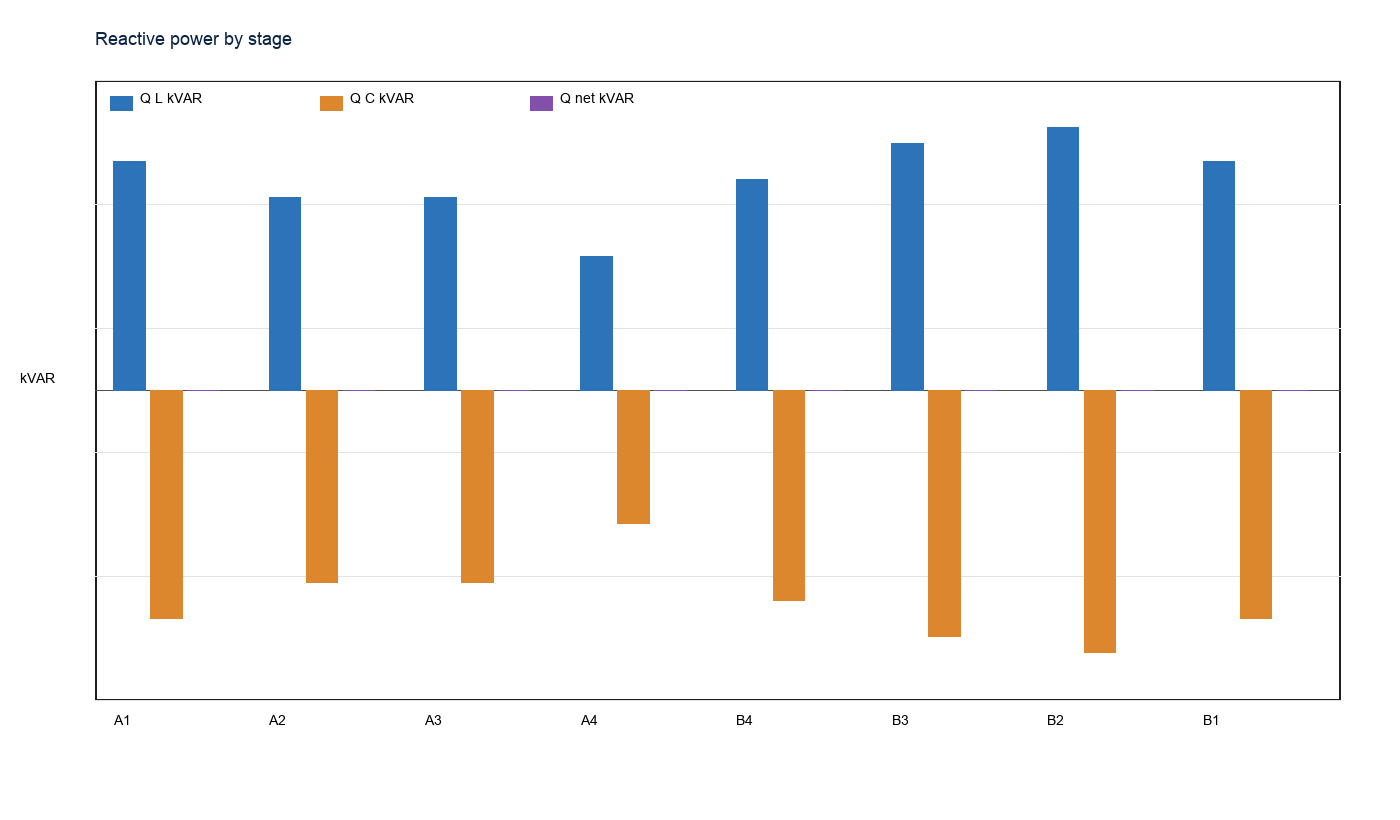
\includegraphics[width=0.94\textwidth]{../figures_updated_coils_20260531/stage_reactive_power.png}
\caption{Updated-coil branch-tank reactive-power balance by stage.}
\label{fig:upd-stage-reactive}
\end{figure}


\section{Metglas AMCC-1000 Results}
The orthogonal AMCC-1000 center is represented by U\_A and U\_B resonators.
At the reference \SI{2}{mm} gap the small-signal model gives the following
core geometry and dynamic response.

\resizebox{0.92\textwidth}{!}{%
\begin{tabular}{lrlrrrr}
\toprule
Part & Orientation & Flux axis & Turns & Gap (mm) & Lself (mH) & XL 128 kHz (ohm) \\
\midrule
U\_A & 0.0 & X & 8 & 2.000 & 0.092052 & 74.032 \\
U\_B & 90.0 & Y & 8 & 2.000 & 0.092052 & 74.032 \\
\bottomrule
\end{tabular}
}

\resizebox{\textwidth}{!}{%
\begin{tabular}{lrrrrrr}
\toprule
Mode & I rms (A) & I pk (A) & Vc rms (V) & B rms (T) & B pk (T) & Damping W \\
\midrule
U\_A & 2.475486 & 3.449532 & 183.252676 & 0.012384 & 0.017257 & 37.806078 \\
U\_B & 3.369183 & 4.758976 & 249.434126 & 0.016855 & 0.023808 & 70.030936 \\
\bottomrule
\end{tabular}
}

\resizebox{\textwidth}{!}{%
\begin{tabular}{lrrl}
\toprule
Metric & RMS/mean & Peak/limit & Unit \\
\midrule
U\_A\_core\_current & 2.478628 & 3.449532 & A \\
U\_B\_core\_current & 3.367880 & 4.758976 & A \\
U\_A\_capacitor\_voltage & 183.020191 & 255.414153 & V \\
U\_B\_capacitor\_voltage & 249.530296 & 352.351148 & V \\
U\_A\_flux\_density & 0.012400 & 0.017257 & T \\
U\_B\_flux\_density & 0.016849 & 0.023808 & T \\
direct\_U\_A\_to\_U\_B\_mutual\_voltage & 14.275697 & 19.908115 & V \\
input\_A4\_to\_U\_A\_mutual\_voltage & 21.629079 & 30.577635 & V \\
output\_U\_B\_to\_B4\_mutual\_voltage & 54.305273 & 76.609354 & V \\
actual\_average\_U\_A\_to\_U\_B\_power & 10.267611 & 58.458069 & W \\
actual\_average\_net\_U\_A\_to\_U\_B\_power & 21.344931 & 22.945421 & W \\
matched\_thevenin\_U\_A\_to\_U\_B\_limit & 8.711158 & 70.991223 & W \\
\bottomrule
\end{tabular}
}


\begin{figure}[H]
\centering
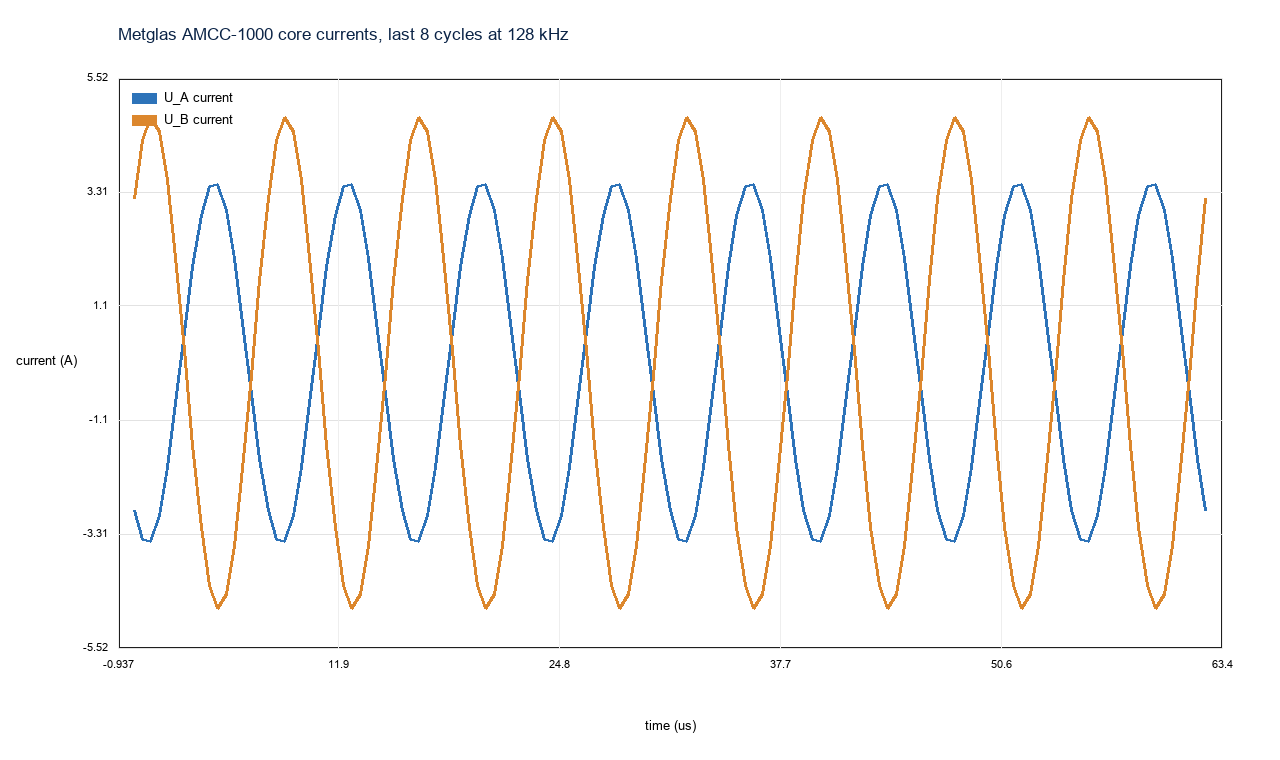
\includegraphics[width=0.94\textwidth]{../figures_updated_coils_20260531/metglas_core_currents.png}
\caption{Updated-coil Metglas $U_A$ and $U_B$ resonant currents over the final eight cycles.}
\label{fig:upd-metglas-currents}
\end{figure}


\begin{figure}[H]
\centering
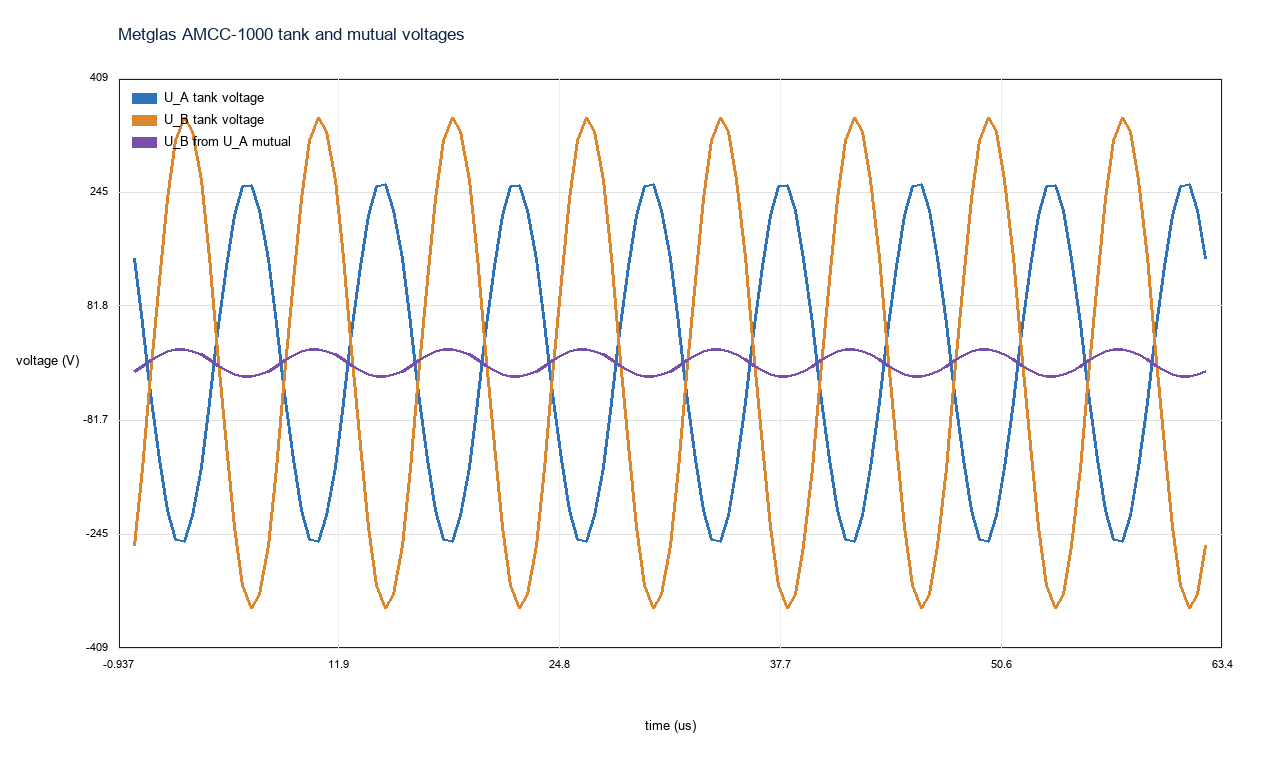
\includegraphics[width=0.94\textwidth]{../figures_updated_coils_20260531/metglas_core_voltages.png}
\caption{Updated-coil Metglas tank voltages and the direct $U_A$ to $U_B$ mutual voltage.}
\label{fig:upd-metglas-voltages}
\end{figure}


\begin{figure}[H]
\centering
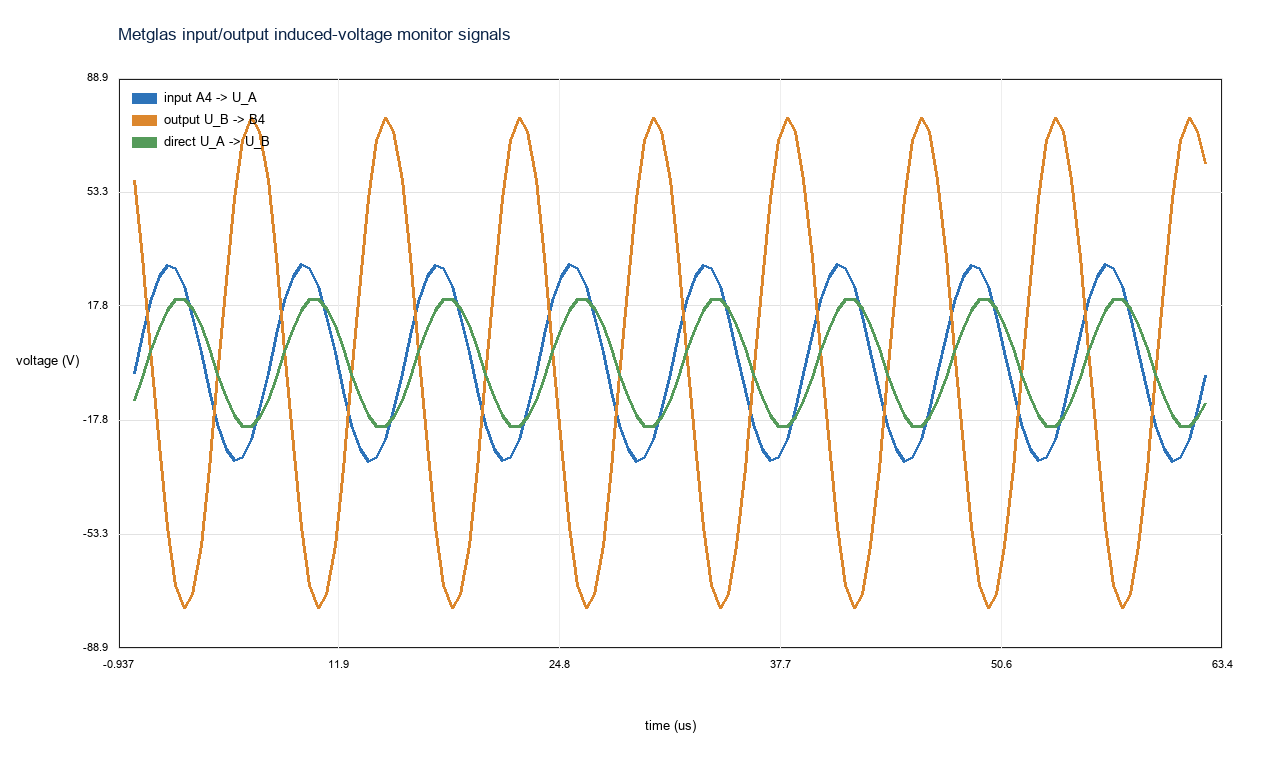
\includegraphics[width=0.94\textwidth]{../figures_updated_coils_20260531/metglas_input_output_signals.png}
\caption{Input and output monitor voltages: A4 into $U_A$, $U_B$ into B4, and direct $U_A$ to $U_B$.}
\label{fig:upd-metglas-io}
\end{figure}


\begin{figure}[H]
\centering
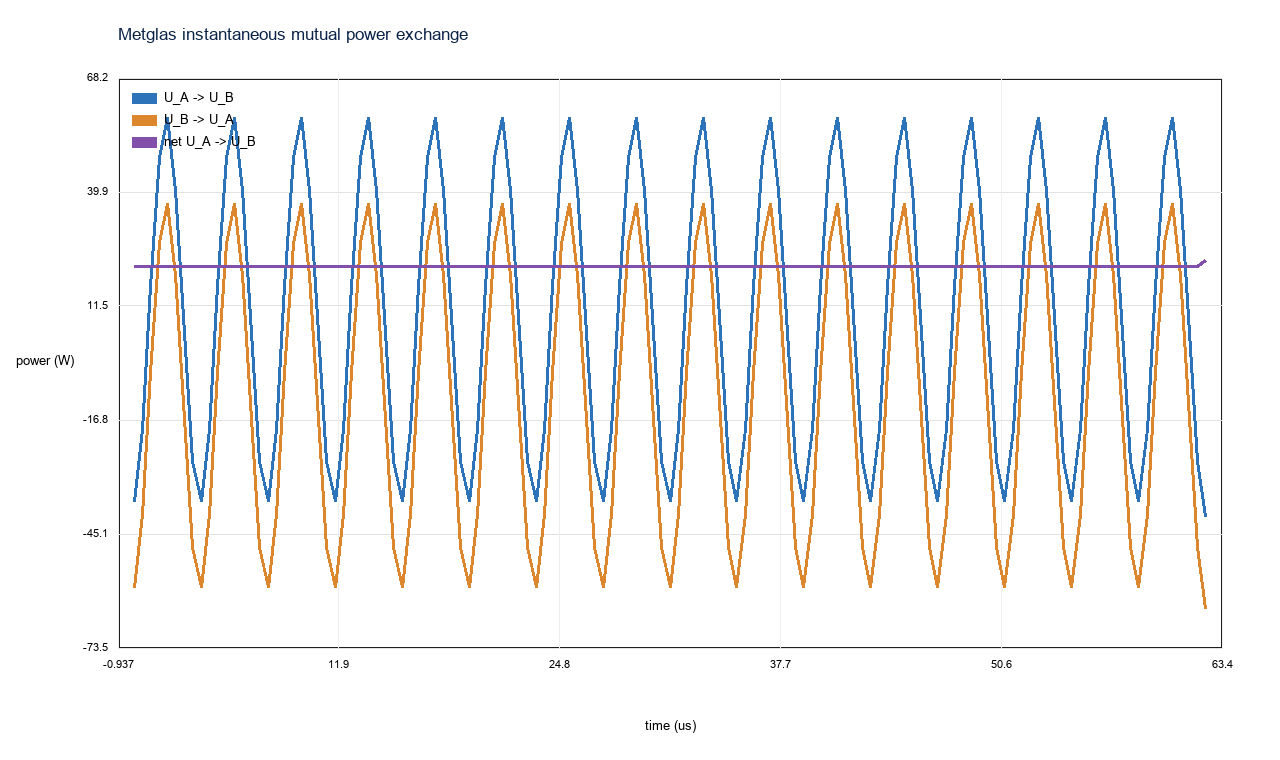
\includegraphics[width=0.94\textwidth]{../figures_updated_coils_20260531/metglas_transferred_power_time.png}
\caption{Instantaneous mutual power exchange and net directional power in the orthogonal Metglas pair.}
\label{fig:upd-metglas-power-time}
\end{figure}


\section{Transfer Limits and Near-10 kW Orthogonal Point}
For a sinusoidal primary current \(I_1\), the open-circuit secondary voltage is
\begin{equation}
V_{2,\mathrm{oc}} = \omega M I_1,
\end{equation}
and the matched-load Thevenin limit is
\begin{equation}
P_{\max} = \frac{V_{2,\mathrm{oc}}^2}{4R_2}.
\end{equation}
With \(k=0.08\), the dynamic-current U\_A to U\_B matched limit is
\SI{8.711158}{W}, while the \SI{50}{mT}
target-current limit is \SI{70.991223}{W}.

\resizebox{\textwidth}{!}{%
\begin{tabular}{lrrrrr}
\toprule
Case & k & M (uH) & Ipri (Arms) & Voc (Vrms) & Pmax (W) \\
\midrule
dynamic\_U\_A\_to\_U\_B & 0.080 & 7.364140 & 2.475577 & 14.661833 & 8.711158 \\
dynamic\_U\_B\_to\_U\_A & 0.080 & 7.364140 & 3.369146 & 19.954079 & 16.134768 \\
target\_50mT\_U\_A\_to\_U\_B & 0.080 & 7.364140 & 7.067092 & 41.855512 & 70.991223 \\
target\_50mT\_U\_B\_to\_U\_A & 0.080 & 7.364140 & 7.067092 & 41.855512 & 70.991223 \\
\bottomrule
\end{tabular}
}


\begin{figure}[H]
\centering
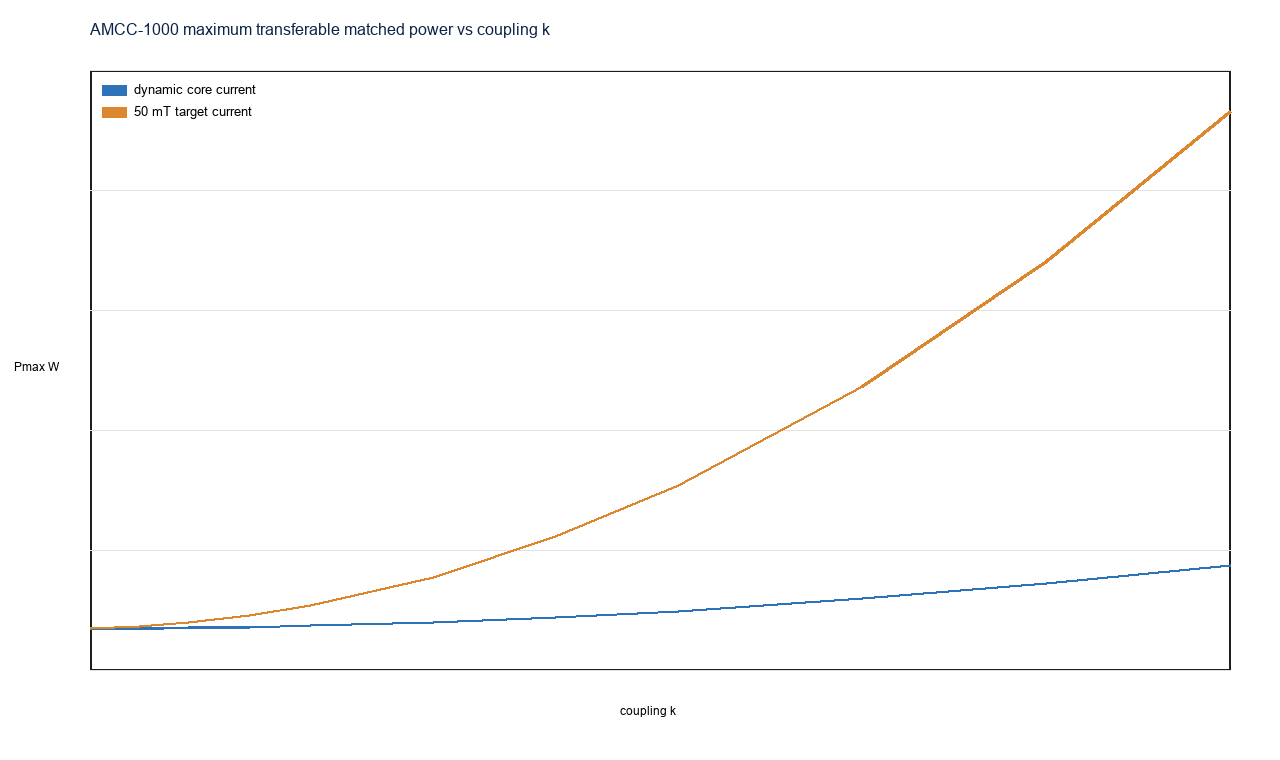
\includegraphics[width=0.94\textwidth]{../figures_updated_coils_20260531/metglas_transfer_power_sweep.png}
\caption{Matched transferable power versus orthogonal coupling coefficient k.}
\label{fig:upd-metglas-transfer-sweep}
\end{figure}


\resizebox{0.88\textwidth}{!}{%
\begin{tabular}{lr}
\toprule
Quantity & Value \\
\midrule
Required B peak & 0.593428 T \\
Selected turns per winding & 12 \\
Primary winding current & 55.917426 Arms \\
Primary winding voltage & 9314.329 Vrms \\
Secondary open-circuit voltage & 745.146 Vrms \\
Matched secondary resistance & 13.881077 ohm \\
Matched secondary current & 26.840365 Arms \\
Matched secondary power & 10000.000 W \\
L self & 0.207116 mH \\
M mutual & 16.569316 uH \\
Resonance C & 7.464586 nF \\
Circulating reactive power & 0.520833 MVAR \\
Parallel AWG10-equivalent bundles & 4 \\
Procurement cable, two windings & 93.840 m \\
\bottomrule
\end{tabular}
}

\section{Interpretation}
The updated coil values remove the former inconsistency between cable length,
turn count, and branch inductance.  The A/B ladder is now internally consistent
at the level of the lumped finite-solenoid model.  The limiting problem remains
the orthogonal Metglas transfer.  Weak coupling at \(k=0.08\) gives only a small
matched transfer under the dynamic currents, while a near-\SI{10}{kW} point
requires \SI{0.593428}{T} peak flux density, \SI{55.917}{A_{rms}},
\SI{9.314}{kV_{rms}}, and about \SI{0.521}{MVAR} of circulating
reactive power.  These are not first-energization conditions; they define an
upper experimental envelope.

\begin{thebibliography}{9}
\bibitem{grover} F. W. Grover, \emph{Inductance Calculations}, Dover Publications.
\bibitem{dowell1966} P. L. Dowell, ``Effects of eddy currents in transformer windings,'' \emph{Proceedings of the IEE}, 1966.
\bibitem{ferreira1992} J. A. Ferreira, ``Analytical computation of AC resistance of round and rectangular litz wire windings,'' \emph{IEE Proceedings B}, 1992.
\bibitem{metglas2605sa1} Metglas Inc., ``2605SA1 Magnetic Alloy,'' product datasheet.
\bibitem{amcc1000} Hitachi Metals / Metglas, ``AMCC1000 product drawing Rev.07.''
\end{thebibliography}

\end{document}
